\chapter{Propuesta de alto nivel}

En este proyecto se tiene como objetivo el diseño y la implementación de un sistema ciberfísico basado en un robot móvil omnidireccional, el cual será utilizado como plataforma para estudiar y modelar el comportamiento de un sistema compuesto por un robot que sigue trayectorias predefinidas calculadas mediante algoritmos de planificación.

La propuesta, por un lado, incluye el desarrollo de un sistema de locomoción omnidireccional compuesto por cuatro ruedas, lo que permitirá al robot moverse en cualquier dirección. Por el otro, se integra una interfaz de usuario para  control y supervisión del comportamiento de los robots.

Para el control global basamos el diseño del sistema en el uso de un conjunto Red de Petri/Monitor. De este modo, el espacio se divide en regiones (discretización) y cada región podrá ser ocupada por un solo robot a la vez.

Para aumentar la precisión en la localización de cada robot dentro del espacio, se agrega el Filtro de Kalman para estimar la posición actual del robot a partir de las lecturas de sus sensores. Al mismo tiempo, el sistema busca resolver desafíos clave de la navegación autónoma, tales como la prevención de colisiones y la mejora de la precisión en la localización del robot dentro de un espacio determinado.

\begin{figure}[H]
    \centering
    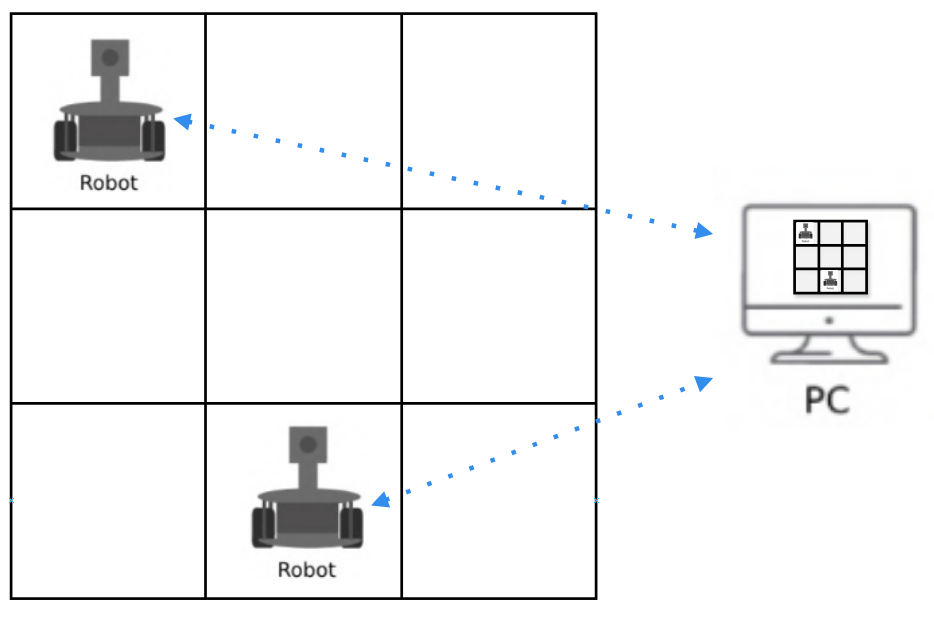
\includegraphics[width=0.65\linewidth]{mt_alto-nivel.png}
    \caption{Propuesta de alto nivel}
    \label{fig:propaltonivel}
\end{figure}

